\chapter{Limits of Direct Reinforcement Learning of Decision Tree Policies}\label{sec:pomdp}

From the previous Chapter~\ref{sec:topin} we know that to directly learn decision trees that directly optimize the RL objective~\ref{def:mdp-obj} for an MDP, one can learn a deterministic partially observable policy for an IBMDP (Definitions~\ref{def:ibmdp} and~\ref{def:irl} and Proposition~\ref{def:po-policy}).
Such problems are classical instances of partially observable Markov decision processes (POMDPs)~\cite{POMDP,chap2}.
This connexion with POMDPs brings novel insights to direct reinforcement learning of decision tree policies. 
In this chapter, all the decision processes presented have a finite number of vector-valued states and observations.
Hence we will use bold fonts for states and observations but can still use summations rather than integrals when required.

\subsection{Partially Observable IBMDPs}\label{sec:poibmdp}
A POMDP is an MDP where the current state is hidden; only some information about the current state is observable.

\begin{definition}[Partially Observable Markov Decision Processes]\label{def:pomdp}
A partially observable Markov decision process is a tuple $\langle X, A, O, T, T_0, \Omega, R\rangle$ where:
\begin{itemize}
    \item $X$ is the state space (like in the definition of MDPs (\ref{def:mdp})).
    \item $A$ is a finite set of actions (like in the definition of MDPs (\ref{def:mdp})).
    \item $O$ is a set of observations.
    \item $T: X \times A \rightarrow \Delta X$ is the transition kernal, where $T(boldsymbol{x}_t, a, \boldsymbol{x}_{t+1}) = P(\boldsymbol{x}_t|\boldsymbol{x}_{t+1}, a)$ is the probability of transitioning to state $\boldsymbol{x}_{t}$ when taking action $a$ in state $\boldsymbol{x}$
    \item $T_0$: is the intial distribution over states. 
    \item $\Omega: X \rightarrow \Delta O$ is the observation kernel, where $\Omega(\boldsymbol{o}, a, \boldsymbol{x}) = P(\boldsymbol{o}|\boldsymbol{x}, a)$ is the probability of observing $\boldsymbol{o}$ in state $\boldsymbol{x}$
    \item $R: X \times A \rightarrow \mathbb{R}$ is the reward function, where $R(\boldsymbol{x}, a)$ is the immediate reward for taking action $a$ in state $\boldsymbol{x}$
\end{itemize}
Note that $\langle X, A, R, T, T_0 \rangle$ defines an MDP (cite).
\end{definition}

Let us define explicitely a partially observable iterative bounding Markove decision process (POIBMDP). It is essentially an IBMDP extended with an observation space and an observation kernel:
\begin{definition}[Partially Observable Iterative Bounding Markov Decision Processes]\label{def:poibmdp} a partially observable iterative bounding Markov decision process $\mathcal{M}_{POIB}$
    \begin{align*}
        \langle \overbrace{S\times \underbrace{O}_{\text{Observations}}}^{\text{full states}}, \underbrace{A\cup A_{info}}_{Action space}, \overbrace{(R, \zeta)}^{Rewards}, \underbrace{(T_{info}, T, T_0)}_{Transitions}, \Omega \rangle
    \end{align*}
    Note that $\langle S\times O, A\cup A_{\info}, (R, \zeta),( T, T_0, T_{info})\rangle$ is an IBMDP~\ref{def:ibmdp}.
    The transition kernel $\Omega$ maps state features and observations to observations, $\Omega:S\times O \rightarrow O$, with $P(\boldsymbol{o}|(\boldsymbol{s}, \boldsymbol{o}))=1$ 
\end{definition}

One can see POIBMDPs as particular instances of POMDPs where the observation kernel simply applies a mask over some features of the full state.
This setting has other names in the litterature.
For example, POIBMDPs are Mixed Observability MDPs \cite{momdp} with base MDP state features as the \textit{hidden variables} and feature bounds as \textit{visible} variables.
POIBMDPs can also be seen as non-stationary MDPs (N-MDPS)~\cite{learning-pomdp} in which there is one different transition kernel per base MDP state: these are called Hidden-Mode MDPs~\cite{hmmdp}. 

Following~\cite{learning-pomdp} we can write the value of a deterministic partially observable policy $\pi:O\rightarrow A\cup A_{info}$ in observation $\boldsymbol{o}$.

\begin{definition}[Partially observable value function]\label{def:vpo} In a POIBMDP (\ref{def:poibmdp}), the expected cumulative discounted reward of a deterministic partially observable policy $\pi:O\rightarrow A\cup A_{info}$ starting from observation $o$ is $V^{\pi}(\boldsymbol{o})$:
    \begin{align*}
        V^{\pi}(\boldsymbol{o}) &= \underset{(s,\boldsymbol{o}')\in S\times O}{\sum}P^{\pi}((\boldsymbol{s}, \boldsymbol{o}')|\boldsymbol{o})V^{\pi}((\boldsymbol{s}, \boldsymbol{o}'))
    \end{align*}
with $P^{\pi}((\boldsymbol{s}, \boldsymbol{o}')|\boldsymbol{o})$ the asymptotic occupancy distribution (see \cite[Section 4]{learning-pomdp} for the full defintion) of the complete POIBMDP state $(\boldsymbol{s},\boldsymbol{o}')$ given the partial observation $o$ and $V^{\pi}((s, o'))$ the classical state-value function defined in (cite).
\end{definition}

The asymptotic occupancy distribution is the probability of a policy $\pi$ to arrive in $(s,\boldsymbol{o}')$ while observing $\boldsymbol{o}$ in some trajectory.  
We can re-write the direct interpretable RL objective (\ref{def:irl}) in terms of POIBMDPs:

\begin{definition}[Revised direct interpretable RL objective]\label{def:revised}
    Given an MDP $\mathcal{M}$ (cite) and an associated POIBMDP $\mathcal{M}_{POIB}$ (\ref{def:poibmdp}), the direct interpretable RL objective becomes:
\begin{align}
    \pi^{\star} &= \underset{\pi}{\operatorname{argmax}}J(\pi) = \underset{\pi}{\operatorname{argmax}}V^{\pi}(\boldsymbol{o}_0)
\end{align}
With $\pi$ a determintic partially observable policy $\pi:O\rightarrow A\cup A_{info}$. There is no expectation over possible initial observation in the above objective function as there is only one initial observation in a POIBMDP: $\boldsymbol{o}_0=(L_1, U_1, \dots, L_n, U_n)$ (c.f. Def.\ref{def:ibmdp}).
\end{definition}
This revised objective is just a re-writing of (\ref{def:irl}) making explicit the POMDP model.
In this Chapter, we use reinforcement learning to train decision tree policies for MDPs by seeking deterministic partially observable policies for POIBMDPs (\ref{def:poibmdp}), i.e. by solving (\ref{def:revised}).
We summarized the approach in Figure~\ref{fig:summary-rl}  

\begin{figure}[h]
\centering
\begin{tikzpicture}
    \draw[fill=blue!40] (0, 0) rectangle (6, 4);
    \node at (3, 3.5) {POIBMDP $\mathcal{M}_{POIB}\langle\mathcal{M}_{IB}, \Omega\rangle$};
    \draw[fill=blue!30] (0, 0) rectangle (5.9, 3);
    \node at (3, 2.5) {IBMDP $\mathcal{M}_{IB} \langle \mathcal{M}, O, A_{info}, \zeta, T_{info}\rangle$};
    \draw[fill=blue!10] (0, 0) rectangle (5, 2);
    \node at (3, 1.5) {MDP $\mathcal{M} \langle S, A, R, T, T_0 \rangle$};
    
    \draw[fill=red!10] (10, 0) rectangle (14, 3);
    \node at (12, 2) {\textbf{Objective~\ref{def:revised}}};
    \node at (12, 1) {$\pi^{\star} = \underset{\pi}{\operatorname{argmax}} V^{\pi}(\boldsymbol{o}_0)$};
    
    \draw[fill=red!10] (1, -5) rectangle (5, -2);
    \node at (3, -3) {\textbf{Decision Tree Policy}};
    \node at (3, -4) {$\pi_{\mathcal{T}}: S \rightarrow A$};
    
    \draw[fill=red!10] (9.5, -5) rectangle (14.5, -2);
    \node at (12, -3) {\textbf{Deterministic policy}};
    \node at (12, -4) {$\pi: O \rightarrow A \cup A_{info}$};
    
    \draw[thick, ->] (6, 2) -- (10, 2) node[midway, above] {$\gamma$};
    \draw[thick, <-] (5, -3.5) -- (9.5, -3.5) node[midway, above] {Extract tree with Alg.\ref{alg:extract-tree}};
    \draw[thick, ->] (12, 0) -- (12, -2) node[midway, left] {Solve with e.g. RL~\ref{sec:rl}};
    \draw[thick, <-] (3, 0.5) -- (3, -2) node[midway, left] {Can be interpreted};

    
    % % Final arrow from tree back to base MDP - adjusted position
    % \draw[thick, ->] (1.75, -2.5) -- (1.75, -0.5) node[midway, right] {Can deploy\\and interpret};
    
\end{tikzpicture}
\caption{A formal framework to learn decision tree policies for MDPs that directly optimize a trade-off between the RL objective~\ref{def:mdp-obj} and interpretability.
This framework relies on learning a partially observable deterministic policy in a POIBMDP~\ref{def:poibmdp}.}
\label{fig:summary-rl}
\end{figure}

We will attempt to \textit{learn} an optimal depth-1 tree policy w.r.t the RL objective (\ref{def:mdp-obj}) for the $2\times 2$ grid world from Example \ref{example:grid}.
One of those two optimal depth-1 tree is given in Figure~\ref{fig:optimal-policy-trees}. The other optimal depth-1 tree is to go right when $y\leq 1$ and down otherwise
We formulate this as solving the (revised) direct interpretble RL objective~\ref{def:revised} where the base MDP is the grid world and the POIBMDP is obtained from the IBMDP of Example \ref{example:ibmdp}.

We choose $\gamma$ and $\zeta$ in the POIBMDP such that the \textit{optimal} partially observable deterministic policy, i.e. the solution to (\ref{def:revised}), corresponds exactly to the decision tree of depth 1 from Figure~\ref{fig:trees-intro}.
This depth 1 tree is in turn optimal in the grid world MDP w.r.t to the base RL objective (\ref{def:mdp-obj}).
Next we present some insights about the solution space of (\ref{def:revised}).

\section{Constructing POIBMDPs which optimal solutions are the depth-1 tree}
\begin{figure}[htbp]
    \centering
    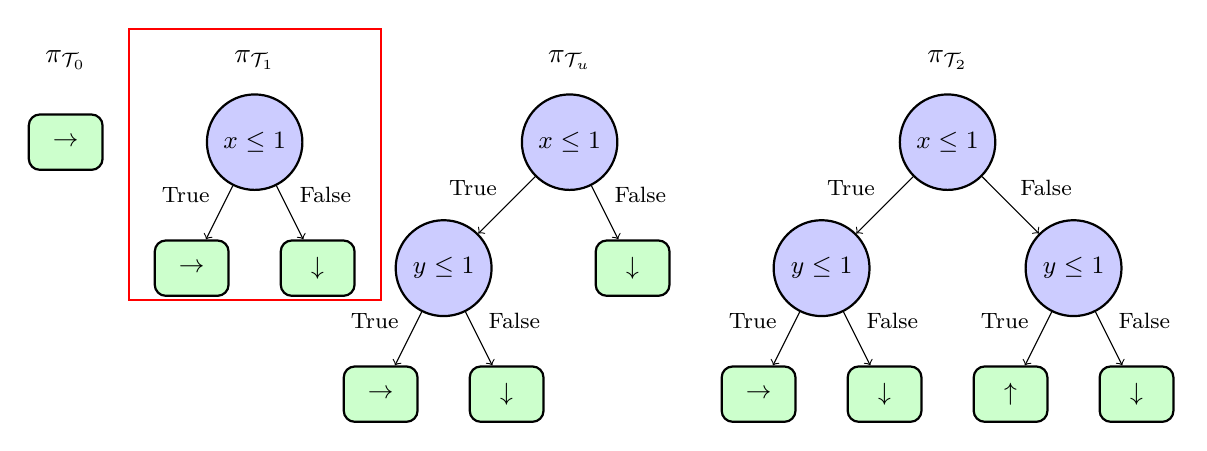
\begin{tikzpicture}[
        scale=0.8,
        decision/.style={circle, draw, thick, fill=blue!20, text width=2.5em, text centered, minimum height=2.5em, font=\small},
        leaf/.style={rectangle, draw, thick, fill=green!20, text width=2em, text centered, rounded corners, minimum height=2em, font=\small},
        edge_label/.style={font=\footnotesize, midway}
    ]
        
        \node[leaf] at (-3, 0) {$\rightarrow$};
        % Tree 4: if x <= 0.5 move right else move left
        \node[decision] (tree4_root) at (0,0) {$x \leq 1$};
        \node[leaf] (tree4_right) at (-1,-2) {$\rightarrow$};
        \node[leaf] (tree4_left) at (1,-2) {$\downarrow$};
        \draw[->] (tree4_root) -- (tree4_right) node[edge_label, above left] {True};
        \draw[->] (tree4_root) -- (tree4_left) node[edge_label, above right] {False};
        
        % Draw a square around the tree
        \draw[thick, red] (-2, 1.8) rectangle (2, -2.5);

        % Tree 7: if x <= 0.5 and y <= 0.5 move right else move down
        \node[decision] (tree7_root) at (5,0) {$x \leq 1$};
        \node[decision] (tree7_y) at (3,-2) {$y \leq 1$};
        \node[leaf] (tree7_right) at (2,-4) {$\rightarrow$};
        \node[leaf] (tree7_down) at (4,-4) {$\downarrow$};
        \node[leaf] (tree7_down2) at (6,-2) {$\downarrow$};
        \draw[->] (tree7_root) -- (tree7_y) node[edge_label, above left] {True};
        \draw[->] (tree7_root) -- (tree7_down2) node[edge_label, above right] {False};
        \draw[->] (tree7_y) -- (tree7_right) node[edge_label, above left] {True};
        \draw[->] (tree7_y) -- (tree7_down) node[edge_label, above right] {False};


        \node[decision] (tree7_root) at (11,0) {$x \leq 1$};
        \node[decision] (tree7_y) at (9,-2) {$y \leq 1$};
        \node[decision] (tree7_y2) at (13,-2) {$y \leq 1$};
        \node[leaf] (tree7_right) at (8,-4) {$\rightarrow$};
        \node[leaf] (tree7_down) at (10,-4) {$\downarrow$};
        \node[leaf] (tree7_right2) at (12,-4) {$\uparrow$};
        \node[leaf] (tree7_down2) at (14,-4) {$\downarrow$};
        \draw[->] (tree7_root) -- (tree7_y) node[edge_label, above left] {True};
        \draw[->] (tree7_root) -- (tree7_y2) node[edge_label, above right] {False};
        \draw[->] (tree7_y) -- (tree7_right) node[edge_label, above left] {True};
        \draw[->] (tree7_y) -- (tree7_down) node[edge_label, above right] {False};
        \draw[->] (tree7_y2) -- (tree7_right2) node[edge_label, above left] {True};
        \draw[->] (tree7_y2) -- (tree7_down2) node[edge_label, above right] {False};

        % Labels
        \node[above] at (-3,1) {$\pi_{\mathcal{T}_0}$};
        \node[above] at (0,1) {$\pi_{\mathcal{T}_1}$};
        \node[above] at (5,1) {$\pi_{\mathcal{T}_u}$};
        \node[above] at (11,1) {$\pi_{\mathcal{T}_2}$};


    \end{tikzpicture}
    \caption{For each decision tree structure, e.g., depth-1 or unbalanced depth-2, we illustrate a decision tree which maximizes the RL objective (\ref{def:mdp-obj}).}
    \label{fig:optimal-policy-trees}
\end{figure}

Because we know all the base states, all the observations, all the actions, all the rewards and all the transitions of our POIBMDP, we can compute exactly the values of different partially observable deterministic policies given $\zeta$ the reward for IGAs and $\gamma$ the discount factor.
Each of those policies can be one of the following trees illustrated in Figure~\ref{fig:optimal-policy-trees}: 

\begin{itemize}
    \item $\pi_{\mathcal{T}_0}$: a depth-0 tree equivalent to always taking the same base action 
    \item $\pi_{\mathcal{T}_1}$: a depth-1 tree equivalent alternating between an IGA and a base action 
    \item $\pi_{\mathcal{T}_u}$: an unbalanced depth-2 tree that sometimes takes two IGAs then a base action and sometimes a an IGA then a base action
    \item $\pi_{\mathcal{T}_2}$: a depth-2 tree that alternates between taking two IGAs and a base action
    \item an inifinite ``tree'' that only takes IGAs
\end{itemize}
Furthermore, because from~\cite{learning-pomdp} we know that for POMDPs, stochastic policies can sometimes get better expected discounted rewards than deterministic policies, we also compute the value of the stochastic policy that alternates between two base actions: $\rightarrow$ and $\downarrow$.
Those two base actions always lead to the goal state (c.f. Figure~\ref{example:grid}) in expectation.

We detail the calculations for the detpth-1 decision tree objective value~\ref{def:revised} and defer the calculations for the other policies to the Appendix~\ref{calcs}.

\begin{proposition}[Depth-1 decision tree objective value] The objective value of the best depth-1 decision tree from Figure~\ref{fig:optimal-policy-trees} is $V^{\pi_{\mathcal{T}_1}}(o_0) = \frac{4\zeta + \gamma + 2\gamma^3 + \gamma^5}{4(1-\gamma^2)}$.
\end{proposition}

\begin{proof} $\pi_{\mathcal{T}_1}$ has one root node that tests $x\leq1$ (respectively $y\leq1$) and two leaf nodes $\rightarrow$ and $\downarrow$. 
To compute $V^\pi_{\mathcal{T}_1}(\boldsymbol{o}_0)$, we compute the values of $\pi_{\mathcal{T}_1}$ in each of the possible startin states $(\boldsymbol{s}_0, \boldsymbol{o}_0), (\boldsymbol{s}_1, \boldsymbol{o}_0), (\boldsymbol{s}_2, \boldsymbol{o}_0), (\boldsymbol{s}_g, \boldsymbol{o}_0)$ and compute the expectation over those. 
At inititalization, when the base state is $\boldsymbol{s}_g = (1.5, 0.5)$, the depth-1 decision tree policy cycles between taking an information gathering action $x\leq1$ and moving down to get a positive reward for which it gets the returns:
\begin{align*}
    V^{\pi_{\mathcal{T}_1}} (\boldsymbol{s}_g, \boldsymbol{o}_0) &= \zeta + \gamma + \gamma^2 \zeta + \gamma^3 \dots \\
    &= \overset{\infty}{\underset{t=0}\sum} \gamma^{2t} \zeta + \overset{\infty}{\underset{t=0}\sum} \gamma^{2t+1} \\
    &= \frac{\zeta + \gamma}{1 - \gamma^2}
\end{align*}
At inititialization, in either of the base states $\boldsymbol{s}_0=(0.5,0.5)$ and $\boldsymbol{s}_2=(1.5, 1.5)$, the value of the depth-1 decision tree policy is the return when taking one information gathering action $x\leq1$, then moving right or down, then following the policy from the goal state $\boldsymbol{s}_g$:
\begin{align*}
    V^{\pi_{\mathcal{T}_1}} (\boldsymbol{s}_0, o_0) &= \zeta + \gamma 0 + \gamma^2 V^{\pi_{\mathcal{T}_1}} (\boldsymbol{s}_g, o_0) \\
    &= \zeta + \gamma^2 V^{\pi_{\mathcal{T}_1}} (\boldsymbol{s}_g, o_0) \\
    &= V^{\pi_{\mathcal{T}_1}} (\boldsymbol{s}_2, o_0)
\end{align*}
Similarly, the value of the best depth-1 decision tree policy in state $\boldsymbol{s}_1=(0.5,1.5)$ is the value of taking one information gathering action then moving right to $\boldsymbol{s}_2$ then following the policy in $\boldsymbol{s}_2$:
\begin{align*}
    V^{\pi_{\mathcal{T}_1}} (\boldsymbol{s}_1, \boldsymbol{o}_0) &= \zeta + \gamma 0 + \gamma^2 V^{\pi_{\mathcal{T}_1}} (\boldsymbol{s}_2, \boldsymbol{o}_0) \\
    &= \zeta + \gamma^2 V^{\pi_{\mathcal{T}_1}} (\boldsymbol{s}_2, o_0) \\
    &= \zeta + \gamma^2 (\zeta + \gamma^2 V^{\pi_{\mathcal{T}_1}} (\boldsymbol{s}_g, o_0)) \\
    &= \zeta + \gamma^2 \zeta + \gamma^4 V^{\pi_{\mathcal{T}_1}} (\boldsymbol{s}_g, o_0)
\end{align*}
Since the probability of being in any base states at initialization given that the agent observe $\boldsymbol{o}_0$ is the probability of being in any base states at initialization, we can write:
\begin{align*}
    V^{\pi_{\mathcal{T}_1}} (\boldsymbol{o}_0) &= \frac{1}{4} V^{\pi_{\mathcal{T}_1}} (\boldsymbol{s}_g, \boldsymbol{o}_0) + \frac{2}{4} V^{\pi_{\mathcal{T}_1}} (\boldsymbol{s}_2, \boldsymbol{o}_0) + \frac{1}{4} V^{\pi_{\mathcal{T}_1}} (\boldsymbol{s}_1, \boldsymbol{o}_0) \\
    &= \frac{1}{4} \frac{\zeta + \gamma}{1 - \gamma^2} + \frac{2}{4} (\zeta + \gamma^2 \frac{\zeta + \gamma}{1 - \gamma^2}) + \frac{1}{4} (\zeta + \gamma^2 \zeta + \gamma^4 \frac{\zeta + \gamma}{1 - \gamma^2}) \\
    &= \frac{1}{4} \frac{\zeta + \gamma}{1 - \gamma^2} + \frac{2}{4} (\frac{\zeta + \gamma ^ 3}{1-\gamma^2}) + \frac{1}{4}(\frac{\zeta+\gamma^5}{1-\gamma^2}) \\
    &= \frac{4\zeta + \gamma + 2\gamma^3 + \gamma^5}{4(1-\gamma^2)}
\end{align*}
\end{proof}
\begin{figure}
    \centering
    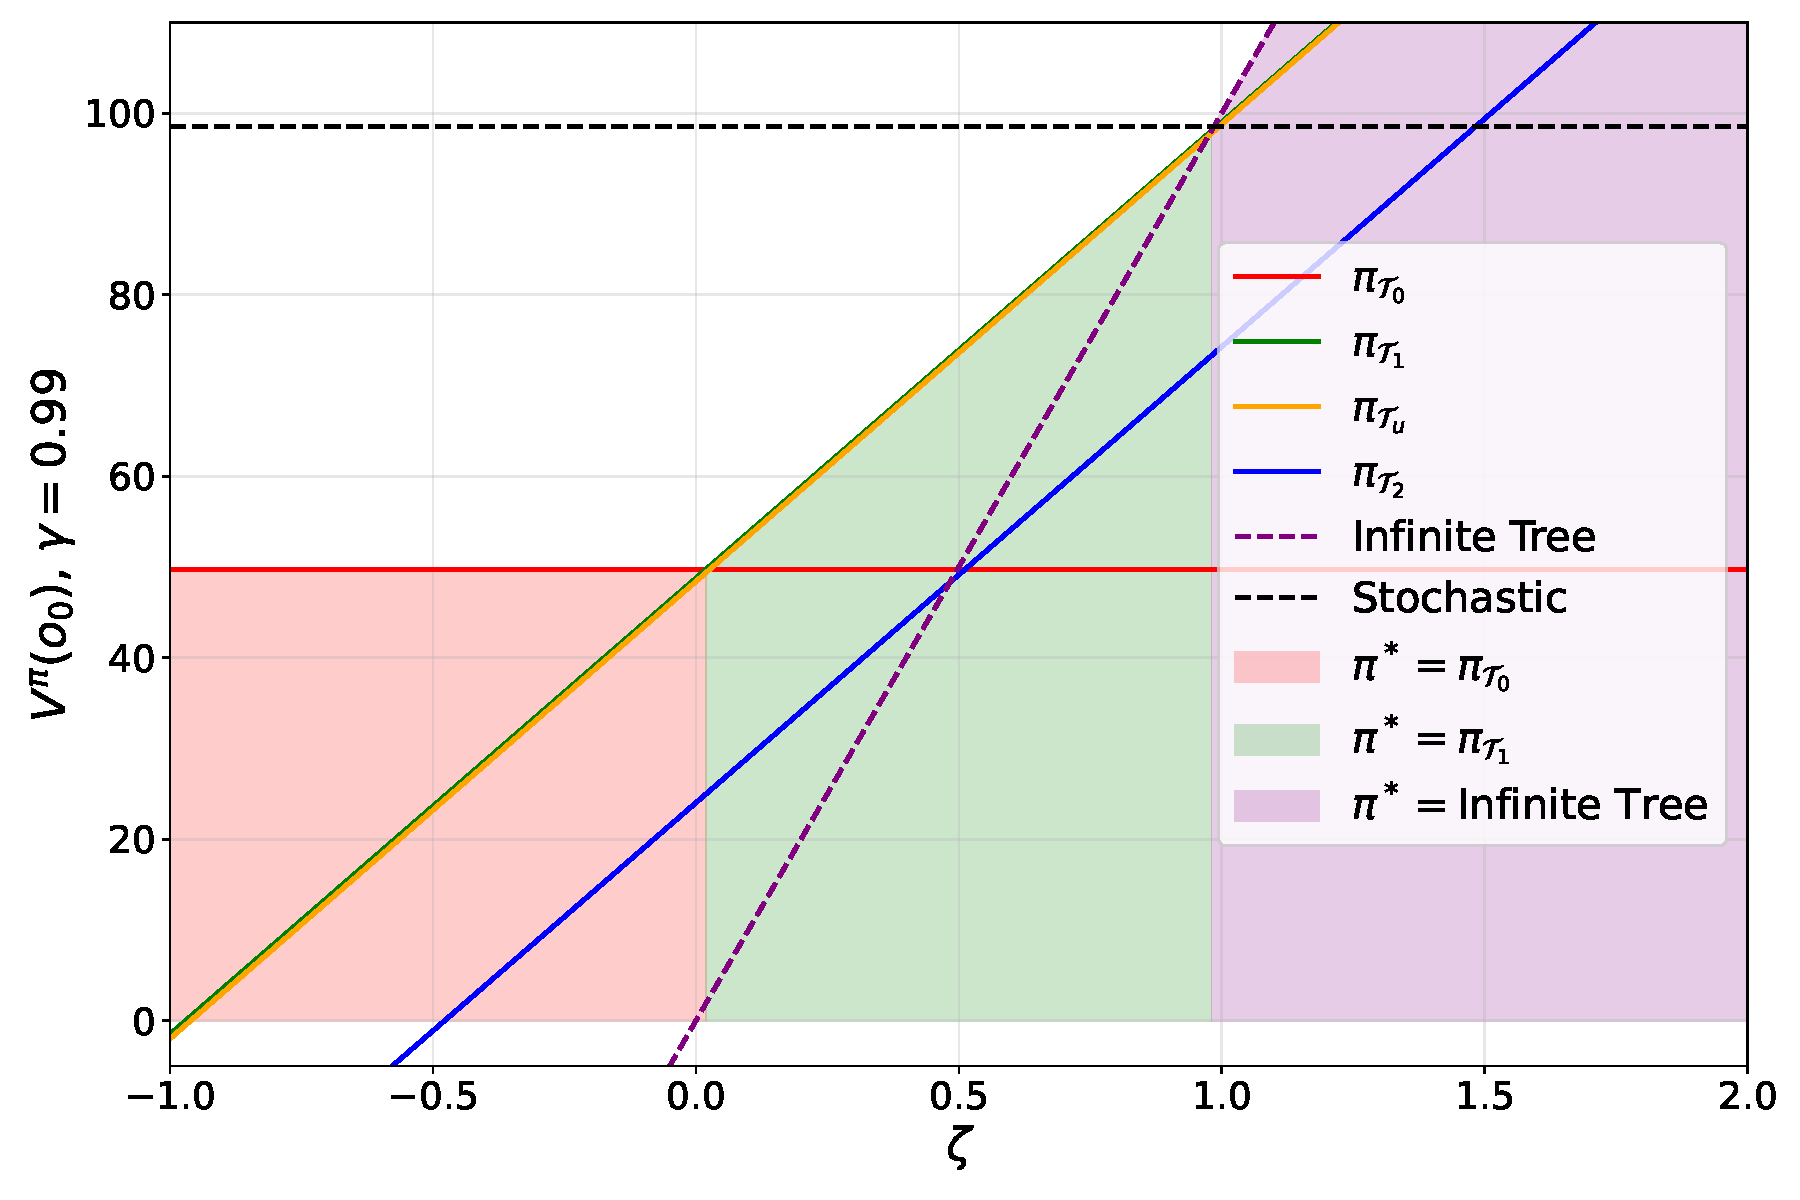
\includegraphics[width=0.6\textwidth]{images/images_part1/objective_values_plot.pdf}
    \caption{POIBMDP objective values of different policies as functions of $\zeta$. Shaded areas show the optimal policies in different ranges of $\zeta$ values.}\label{fig:objectives}
\end{figure}

We can now plot, in Figure~\ref{fig:objectives}, the POIBMDP objective values of the different policies corresponding to trees for the grid world MDP as functions of $\zeta$ when we fix $\gamma=0.99$. 
When $\gamma=0.99$ on Figure~\ref{fig:objectives}, despite objective values being very similar for the depth-1 and unbalanced depth-2 tree, we now know from the green shaded area {\color{blue}a depth-1 tree is the optimal deterministic partially observable POIBMDP policy for $0< \zeta < 1$}.

Interestingly, two POMDP challenges described in \cite{learning-pomdp} can already be observed in Figure~\ref{fig:objectives}. 
First, there is a whole range of $\zeta$ values for which the stochastic policy is optimal.
Second, for e.g. $\zeta=0.5$, while a depth-1 tree is the optimal deterministic partially observable policy, the value of state $(\boldsymbol{s}_2, \boldsymbol{o}_0) = (1.5, 1.5, 0, 2, 0, 2)$ is not maximized by this policy but by the sub-optimal policy that always goes down.

We can now define a POIBMDP with the grid wolrd (\ref{example:grid}) as the base MDP, with IGAs as in the IBMDP from Exapmle~\ref{example:ibmdp}, with $\gamma=0.99$ and $0<\zeta<1$ and verify if RL can retrieve the optimal depth-1 decision tree in this very controlled experiment.

\subsection{Reinforcement Learning in PO(IB)MDPs}

In general, the policy that maximizes the expected discounted cumulative reward in a POMDP maps ``belief states'' or observations histories~\cite{chap2} to actions, i.e., those policies are not solutions to our problem since we require that policies depend only on the current observation.
If we did not have this constraint, we could apply any standard RL algorithm to solve POIBMDPs by seeking such policies because both histories and belief states are sufficient statistic for POMDPs full states~\cite{chap2,lambrechts2025informed}.

The particular, the problem of finding the optimal deterministic partially observable policies for POMDPs is NP-HARD, even with full knowledge of transitions and rewards~\cite[Section 3.2]{littman1}. 

It means that, there is no reason to believe that any algorithm for solving it must enumerate all possible policies and take the best one. 
For even moderate-sized POMDPs, a brute-force approach will take a very long time since there are $|A|^{|O|}$ policies.

Hence it is interesting to study reinforcement learning for finding the best deterministic partially observable policy since it would not search the whole solution space.
However applying RL to our revised interpretable RL objective (\ref{def:revised}) is non-trivial.

In~\cite[Fact 2]{learning-pomdp}, authors show that the optimal partially observable policy can be stochastic, hence policy gradient algoriothms~\cite{pg_sutton} are to prohibit since we want a \textit{deterministic} policy. 
Furthermore, the optimal deterministic patially observable policy might not maximize all the values of all observations simulataneously ~\cite[Fact 5]{learning-pomdp} which makes difficult to use TD-learning to learn policies.
Indeed, doing a TD-learning update of one partially observable value~\ref{def:vpo} with, e.g. Q-learning, can change the value of \textit{all} other observations in a unctrollable manner because of the depedence in $P^{\pi}((s, \boldsymbol{o}')|\boldsymbol{o})$.

Despite those hardness results, empirical results of applying RL to POMDPs by naively replacing $\boldsymbol{x}$ by $\boldsymbol{o}$ in Q-learning or Sarsa, has already demonstrated successful in practice~\cite{sarsa-pomdp}. 
More recently, the framework of Baisero et. al. called asymmetric RL~\cite{baisero-dqn,baisero-ppo} has also shown promising results to learn POMDP solutions.
Asymmetric RL trains a full-state-dependent model and a history-dependent (or observation-dependent) model informed by the former.
The history-dependent (or observation-dependent) model can thus be deplyed in the POMDP after training since it does not require access to the hidden full state to output actions.
In Algorithms~\ref{alg:asymqlearning} and~\ref{alg:asymsarsa} we present asymmetric Q-learning and asymmetric Sarsa. Given a POMDP, both train an observation-dependet Q-function $Q:O\times A\rightarrow\mathbb{R}$ and a state-dependent Q-function $U:X\times A\rightarrow\mathbb{R}$.

In~\cite{jsj}, authors introduce a policy search algorithm~\ref{sec:rl} that learns a (stochastic) policy $\pi:O\rightarrow\Delta A$ and a critic $V:X\rightarrow \mathbb{R}$ using Monte Carlo estimates to guide policy improvement.
We write this algorithm that we call JSJ (for the authors name Jaakkola, Singh, Jordan) in Algorithm~\ref{alg:jsj}. JSJ is equivalent to a tabular asymmetric policy gradient algorithm (c.f. Alg.~\ref{alg:reinforce}). 

Until recently, the benefits of asymmetric RL over standard RL was only shown empirically and only for history-dependent models.
The work of Gaspard Lambrechts~\cite{justif-asym} proves that some asymmetric RL algorithms learn better history-dependent \textbf{or} observation-dependent policies for solving POMDPs.
This is exactly what we wish for. However, those algorithms are intractable in practice because they require estimation of the quantity $P^{\pi}((s, \boldsymbol{o}')|\boldsymbol{o})$ (\ref{def:vpo}).
We leave it to future work to use those algorithms that combine asymmetric RL and estimation of future visitations since those results are contemporary to the writing of this manuscript.

Note that, in the previous chapter, modified DQN (\ref{alg:mod-dqn}) and modified PPO (\ref{alg:mod-ppo}) are respectively asymmetric DQN and asymmetric PPO from~\cite{baisero-dqn,baisero-ppo}.

In the next section, we use (asymmetric) RL to learn decision tree policies for the grid world MDP (\ref{example:grid}).

\RestyleAlgo{ruled}
\SetKwComment{Comment}{}{}
\begin{algorithm}
    \KwData{POMDP $\mathcal{M}_{po} = \langle X, O, A, R, T, T_0, \Omega \rangle$, learning rates $\alpha_u,\quad \alpha_q$, exploration rate $\epsilon$}
    \KwResult{$\pi:O\rightarrow A$}
    Initialize $U(x,a) = 0$ for all $x \in X, a \in A$ \\
    Initialize $Q(o,a) = 0$ for all $o \in O, a \in A$ \\

    \For{each episode}{
        Initialize state $x_0 \sim T_0$ \\
        Initialize observation $\boldsymbol{o}_0 \sim \Omega(x_0)$ \\

        \For{each step $t$}{
            Choose action $a_t$ using $\epsilon$-greedy: $a_t = \arg\max_a Q(\boldsymbol{o}_t,a)$ with prob. $1-\epsilon$ \\
            Take action $a_t$, observe $r_t = R(x_t,a_t)$, $x_{t+1} \sim T(x_t,a_t)$, and $\boldsymbol{o}_{t+1} \sim \Omega(x_{t+1})$ \\
            $y \leftarrow r + \gamma U(x_{t+1}, \argmax_{a'} Q(\boldsymbol{o}_{t+1}, a'))$ \Comment{// TD target} \\
            $U(x_t,a_t) \leftarrow (1 - \alpha_u) U(x_t, a_t) + \alpha_u y $ \\
            $Q(\boldsymbol{o}_t,a_t) \leftarrow (1 - \alpha_q) Q(\boldsymbol{o}_t, a_t) + \alpha_q y $ \\
            $x_t \leftarrow x_{t+1}$ \\
            $\boldsymbol{o}_t \leftarrow \boldsymbol{o}_{t+1}$ \\
        }
    }
    $\pi(o) = \arg\max_a Q(o,a)$ \Comment{// Extract greedy policy}
    \caption{Asymmetric Q-Learning}\label{alg:asymqlearning}
\end{algorithm}


\RestyleAlgo{ruled}
\SetKwComment{Comment}{}{}
\begin{algorithm}
    \KwData{POMDP $\mathcal{M}_{po} = \langle X, O, A, R, T, T_0, \Omega \rangle$, learning rates $\alpha_u,\quad \alpha_q$, exploration rate $\epsilon$}
    \KwResult{$\pi:O\rightarrow A$}
    Initialize $U(x,a) = 0$ for all $x \in X, a \in A$ \\
    Initialize $Q(o,a) = 0$ for all $o \in O, a \in A$ \\

    \For{each episode}{
        Initialize state $x_0 \sim T_0$ \\
        Initialize observation $\boldsymbol{o}_0 \sim \Omega(x_0)$ \\
        Choose action $a_0$ using $\epsilon$-greedy: $a_0 = \arg\max_a Q(\boldsymbol{o}_0,a)$ with prob. $1-\epsilon$ \\

        \For{each step $t$}{
            Take action $a_t$, observe $r_t = R(x_t,a_t)$, $x_{t+1} \sim T(x_t,a_t)$, and $\boldsymbol{o}_{t+1} \sim \Omega(x_{t+1})$ \\
            Choose action $a_{t+1}$ using $\epsilon$-greedy: $a_{t+1} = \arg\max_a Q(\boldsymbol{o}_{t+1},a)$ with prob. $1-\epsilon$ \\
            $y \leftarrow r + \gamma U(x_{t+1}, a_{t+1})$ \Comment{// TD target using actual next action} \\
            $U(x_t,a_t) \leftarrow (1 - \alpha_u) U(x_t, a_t) + \alpha_u y $ \\
            $Q(\boldsymbol{o}_t,a_t) \leftarrow (1 - \alpha_q) Q(\boldsymbol{o}_t, a_t) + \alpha_q y $ \\
            $x_t \leftarrow x_{t+1}$ \\
            $\boldsymbol{o}_t \leftarrow \boldsymbol{o}_{t+1}$ \\
            $a_t \leftarrow a_{t+1}$ \\
        }
    }
    $\pi(o) = \arg\max_a Q(o,a)$ \Comment{// Extract greedy policy}
    \caption{Asymmetric Sarsa}\label{alg:asymsarsa}
\end{algorithm}

\RestyleAlgo{ruled}
\SetKwComment{Comment}{}{}
\begin{algorithm}
    \KwData{POMDP $\mathcal{M}_{po} = \langle X, O, A, R, T, T_0, \Omega \rangle$, learning rate $\alpha$, policy parameters $\theta$, number of trajectories $N$}
    \KwResult{Stochastic partially observable policy $\pi_\theta: O\rightarrow \Delta A$}
    Initialize policy parameters $\theta$ \\
    Initialize $Q(o, a) = 0$ for all observations $o$ and actions $a$ \\
    \For{each episode}{
        \For{$i = 1$ to $N$}{
            Generate trajectory $\tau_i = (\boldsymbol{s}_0, a_0, r_0, \boldsymbol{s}_1, a_1, r_1, \ldots, \boldsymbol{s}_T)$ following $\pi_\theta$ \\
            \For{each timestep $t$ in trajectory $\tau_i$}{
                $G_t \leftarrow \sum_{k=t}^{T} \gamma^{k-t} r_k$ \Comment{// Compute return}
                Store $(\boldsymbol{o}_t, a_t, G_t)$ for later averaging
            }
        }
        \For{each unique observation-action pair $(o, a)$}{
            $Q(o, a) \leftarrow \frac{1}{|\{(o, a)\}|} \sum_{(o, a, G)} G$ \Comment{// Monte Carlo estimate}
        }
        \For{each observation $o$}{
            \For{each action $a$}{
                $\pi_1(a|o) \leftarrow 1.0$ if $a = \argmax_{a'} Q(o, a')$, $0.0$ otherwise \Comment{// Deterministic policy from Q-values}
                $\pi(a|o) \leftarrow (1 - \alpha) \pi(a|o) + \alpha \pi_1(a|o)$ \Comment{// Policy improvement step}
            }
        }
        Reset $Q(o, a) = 0$ for all observations $o$ and actions $a$ \Comment{// Reset for next episode}
    }
    \caption{JSJ algorithm. Uses Monte Carlo estimates of the average reawrd value functions to perform policy imporvements}\label{alg:jsj}
\end{algorithm}

\section{Results}

Unfortunately, our results are negative and show that (asymmetric) reinforcement learning fails for the aforementioned problem. Let us understand why.

\subsection{Experimental Setup}

\paragraph{Baselines:} we consider two groups of RL algorithms.
The first group is standard tabular RL naively applied to POIBMDPs; Q-learning, Sarsa, and Policy Gradient with a softmax policy (c.f. Sec.~\ref{sec:rl}).
In theory the Policy Gradient algorithm should not be a good candidate for our problem since it searches for stochastic policies that we showed can be better than our seeked depth-1 decision tree policy (c.f. Figure (cite)).

In addition to the traditional tabular RL algorithms above, we also apply asymmetric Q-learning, asymmetric Sarsa, and JSJ (Algorithms~\ref{alg:asymqlearning},~\ref{alg:asymsarsa} and~\ref{alg:jsj}).
We use at least 200 000 POIBMDP time steps per experiment. Each experiment, i.e an RL algorithm learning in a POIBMDP, is repeated 100 times.  

\paragraph{Hyperparameters:} For all baselines we use, when applicable, exploration rates $\epsilon=0.3$ and learning rates $\alpha=0.1$.

\paragraph{Metrics:} we will consider two metrics.
First, the sub-optimality gap during training of the learned partially observable policy value with respect to the optimal deterministic partially observable POIBMP policy: $|V^\pi^{\star}(\boldsymbol{o}_0) - V^\pi(\boldsymbol{o}_0)|$
Because we know the whole POIBMDP model that we can represent exactly as tables; and because we know for each $\zeta$ the POIBMDP objective value of the optimal partially observable policy (c.f. Figure); we can report the \textit{exact} sub-optimality gaps.

Second, we consider the distribution of the learned trees over the 100 training seeds.
Indeed, since for every POIBMDP we run each algorihtm 100 times, at the end of training we get 100 partially observable deterministic policies (we compute the greedy policy for stochastic policies returned by JSJ and Policy Gradient), from which we can extract the equivalent 100 decision tree policies using Algorithm~\ref{alg:extract-tree} and we can count which one are of e.g. depth-1.
This helps understand which trees RL algorithms tend to learn.

\subsection{Can (asymmetric) RL retrieve optimal deterministic partially observable POIBMDP policies?}

In Figure~\ref{fig:rl-poibmdp}, we plot the sub-optimality gaps--averaged over 100 seeds--of learned policies during training.
We do so for 200 different POIBMDPs where we change the reward for information gathering actions: we sample 200 $\zeta$ values uniformily in $[-1, 2]$.
In Figure~\ref{fig:rl-poibmdp}, a different color represents a different POIBMDP.

Recall from Figure~\ref{fig:objectives} that for:
\begin{itemize}
    \item $\zeta\in [-1, 0]$, the optimal deterministic partiall observable policy is a depth-0 tree
    \item $\zeta\in ]0, 1[$, the optimal deterministic partiall observable is a depth-1 tree
    \item $\zeta\in [1, 2]$, the optimal deterministic partiall observable is a ``inifnite'' tree that contains infinite number of internal nodes.
\end{itemize}
We observe that, despite all experiments converging, independently of the $\zeta$ values, not all algorithms in all POIBMDPs fully minimize the sub-optimality gap.
In particular, all algorithms seem to consistantly minimze the gap, i.e. learn the optimal policy or Q-function, only for $\zeta \in [1, 2]$ (all the yellow lines go to 0).
However, we are interested in the range $\zeta\in ]0, 1[$ where the optimal decision tree is not taking the same action forever.
In that range, no baseline consistently minimizes the sub-optimality gap.


In Figure~\ref{fig:dt-distrib-poibmdp}, we plot the distributions over the final learned trees in function of $\zeta$ from the above runs.
For example, in Figure~\ref{fig:dt-distrib-poibmdp}, in the top left plot, when learning 100 times in a POIBMP with $\zeta=0.5$, Q-learning returned almost 100 times a depth 0 tree.
Again, on none of those subplots do we see a high rate of learned depth-1 trees for $\zeta\in ]0, 1[$.
It is alerting that the most frequent learned trees are the depth-0 trees for $\zeta\in ]0, 1[$ because such trees are way more sub-optimal w.r.t to (\ref{def:revised}) than e.g. the depth-2 unbalanced trees (c.f. Figure~\ref{fig:objectives}).  
One interpretation of this phenomenon is that the learning in POIBMDPs is very difficult and so agents tend to converge to trivial policies, e.g., repeating the same base action.

However, on the positive side, we observe that asymmetric versions of Q-learning and Sarsa have found the optimal policy, the depth-1 decision tree, more frequently throught the optimality range $]0,1[$ than their symmetric counter-parts for $\zeta\in ]0, 1[$.
Next, we quantify how difficult it is to do RL to learn partially observable policies in POIBMDPs.

\begin{figure}
    \centering
    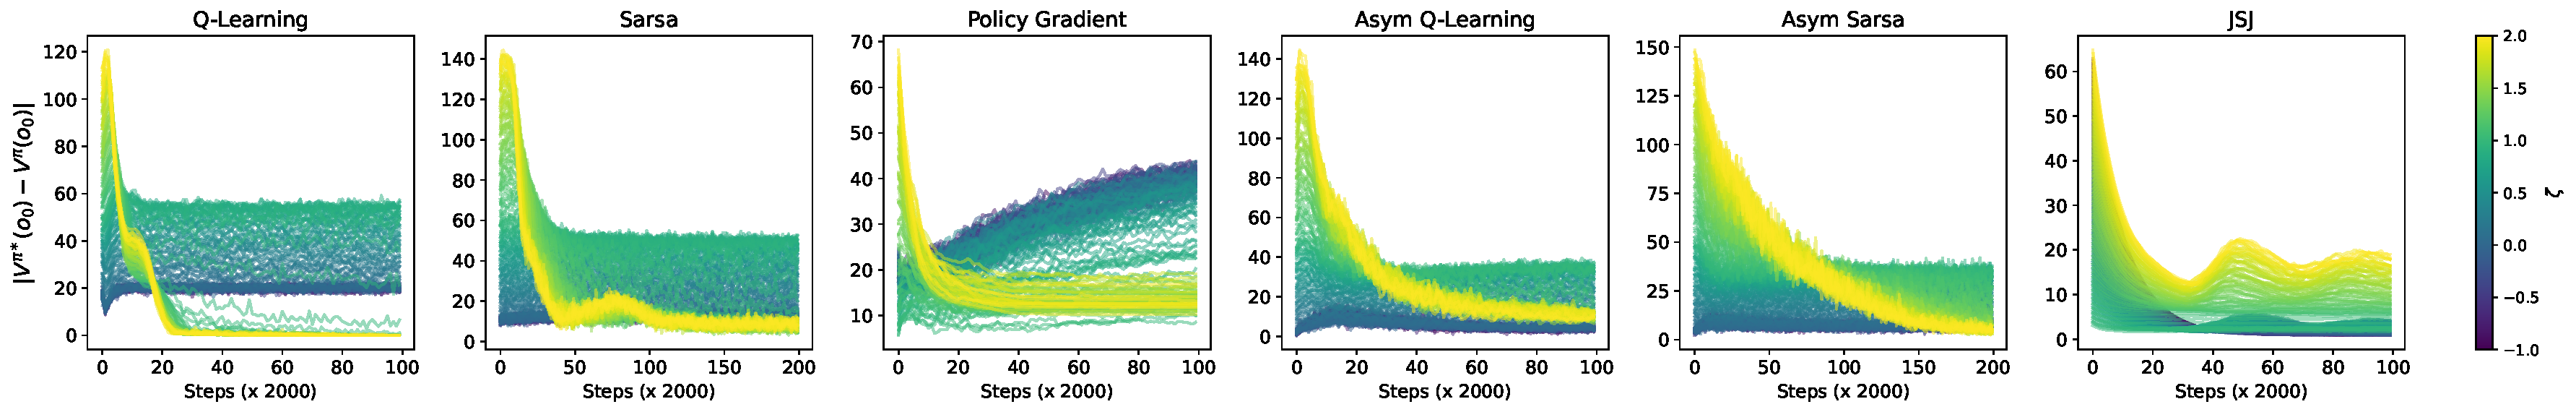
\includegraphics[width=1\textwidth]{images/images_part1/learning_curves.pdf}
    \caption{(Asymmetric) reinforcement learning in POIBMDPs. 
    In each subplot, each single line is colored by the value of $\zeta$ in the corresponding POIBMDP in which learning occurs. 
    Each single learning curve represent the sub-optimality gap averaged over 100 seeds.
    }\label{fig:rl-poibmdp}
\end{figure}

\begin{figure}
    \centering
    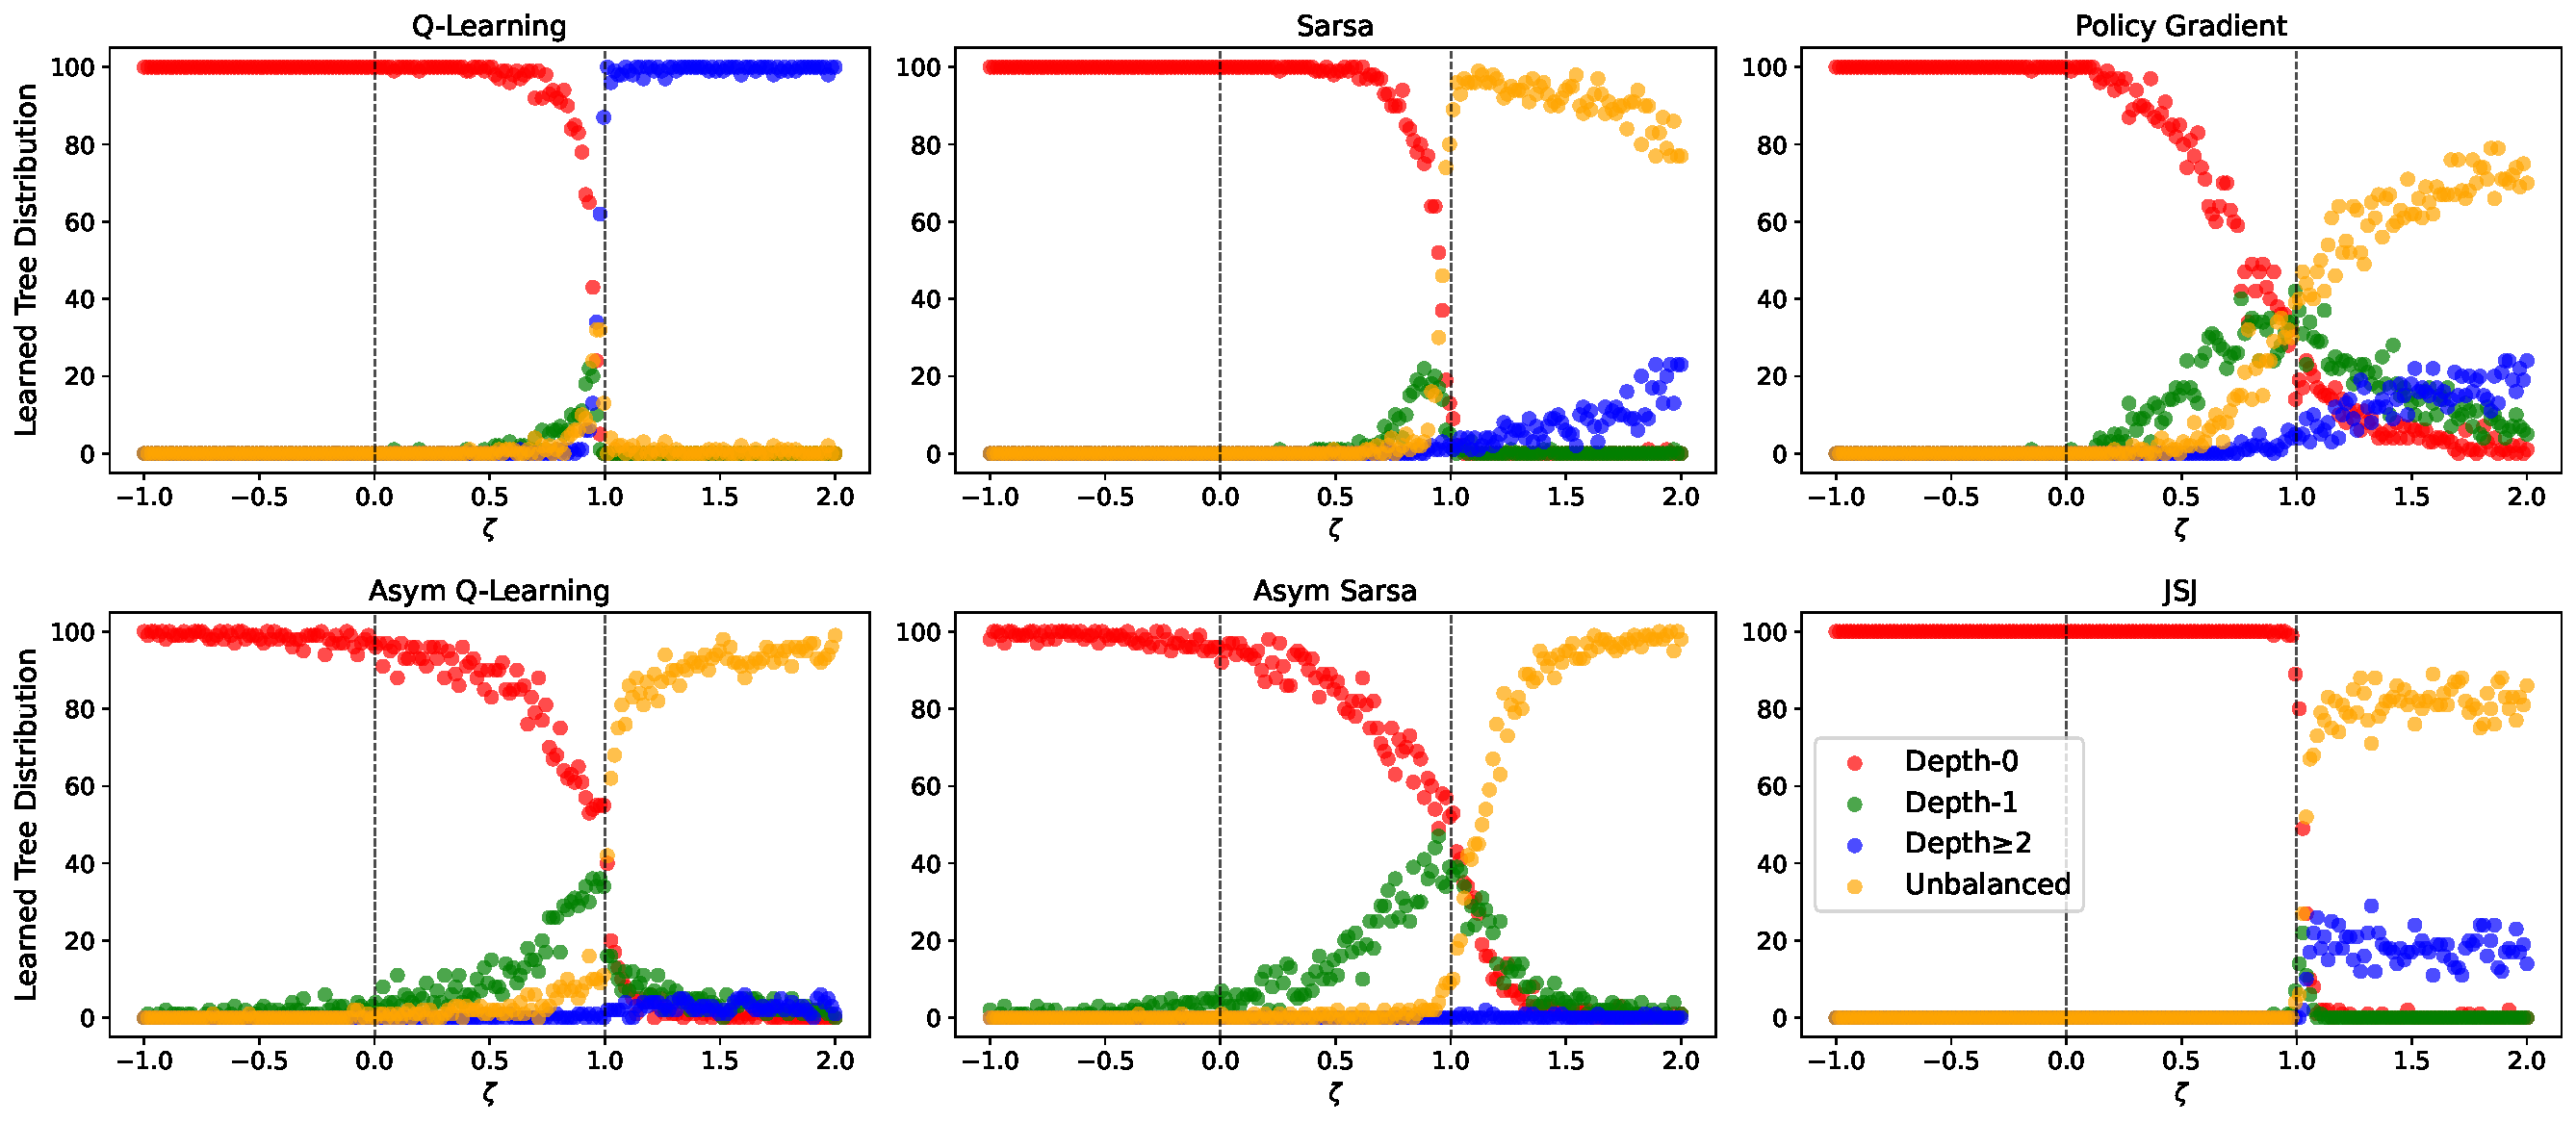
\includegraphics[width=1\textwidth]{images/images_part1/tree_distributions.pdf}
    \caption{Distributions of final tree policies learned across the 100 seeds.
    For each $\zeta$ value, there are four colored points. Each point represent the share of depth-0 trees (red), depth-1 trees (green), unbalanced depth-2 trees (orange) and depth-2 trees (blue).
    }\label{fig:dt-distrib-poibmdp}
\end{figure}


\subsection{How difficult is it to learn in POIBMDPs?}

In this section we run the same (asymmetric) reinforcement learning algorithms to optimize either the RL objective (\ref{def:mdp-obj}) in MDPs (\ref{def:mdp}) or IBMDPs (\ref{def:ibmdp}), or the interpretable RL objective in POIBMDPs~\ref{def:revised}.
This essentially results in three disctint problems:
\begin{enumerate}
    \item Learning an optimal deterministic state-dependent policy in MDPs.
    \item Learning an optimal deterministic full-state-dependent policy in IBMDPs.
    \item Learning an optimal deterministic partially observable policy in POIBMDPs.
\end{enumerate}

In order to see how difficult each of these three problems is, we can run a \textit{big} number of experiments on each and compare success rates.
To make success rates comparable we consider a unique instance for each of those problems.
Problem 1., is learning one of the optimal policy from Figure~\ref{example:grid} for the grid world from Example~\ref{example:grid} with $\gamma=0.99$.
Problem 2., is learning one deterministic optimal policy for the IBMDP from Figure~\ref{example:ibmdp} with $\gamma=0.99$ and $\zeta=0.5$.
This is similar to the previous chapter's experiments where we applied DQN or PPO to the IBMDP for CartPole without constraining the search to partially observable policies (see e.g. Fig.\ref{fig:res-ppo}).
Problem 3. is what has been done in the previous section where in addition of fixing $\gamma=0.99$ we also fix $\zeta=0.5$.

We use the six (asymmetric) RL algoroithms from the previous section and try a wide set of hyperparameters and additional learning tricks (optimistic Q-function, eligibility traces, entropy regularization and $\epsilon$-decay, all are described in \cite{sutton}).
We only provide the detailed hyperparameters for asymmetric Sarsa and a an overall summary for all the algorithms.
The complete detailed lists of hyperparameters are given in the Appendix~\ref{sec:hp-pomdp}.
Furhtermore, the careful reader might notice that there is no point running asymmetric RL on MDPs or IBMDPs when the problem does not require partial observability.
Hence, we only run asymmetric RL for POIBMDPs and otherwise run all other RL algorithms and all problems.

Each unique hyperparameters combination for a given algorithm on a given problem is run 10 times on 1 million learning steps.
For example, for asymmetric Sarsa, we run a total of $10\times 768= 7680$ experiments for learning partially observable deterministic policies for a POIBMDP (c.f. Table~\ref{tab:hp-sarsa}).
To get a success rate, we can simply divide the number of learned depth 1 tree by 7680 (recall that for $\gamma=0.99$ and $\zeta=0.5$, the optimal policy is a depth-1 tree (e.g. Figure~\ref{fig:optimal-policy-trees}) as per Figure~\ref{fig:objectives}). 

\begin{table}[h]
\centering
\small
\caption{Asymmetric Sarsa Hyperparameter Space (768 combinations each run 10 times)}\label{tab:hp-sarsa}
\begin{tabular}{lll}
\toprule
\textbf{Hyperparameter} & \textbf{Values} & \textbf{Description} \\
\midrule
Epsilon Schedules & (0.3, 1), (0.3, 0.99), (1, 1) & Initial exploration and decrease rate \\
Epsilon Schedules & (0.1, 1), (0.1, 0.99), (0.3, 0.99) & Initial exploration and decrease rate \\
Lambda & 0.0, 0.3, 0.6, 0.9 & Eligibility trace decay \\
Learning Rate $U$ & 0.001, 0.005, 0.01, 0.1 & learning rate for \\
 & & the full-state-dependent Q-function \\
Learning Rate $Q$ & 0.001, 0.005, 0.01, 0.1 & learning rate for the \\
 & & partial observation dependent Q-function \\
Optimistic & True, False & Optimistic initialization \\
\bottomrule
\end{tabular}
\end{table}

\begin{table}[h]
    \centering
    \caption{Summary of RL baselines Hyperparameters}
    \begin{tabular}{llr}
    \toprule
    \textbf{Algorithm} & \textbf{Problem} & \textbf{Total Hyperparameter Combinations} \\
    \midrule
    Policy Gradient & PO/IB/MDP & 420 \\
    JSJ & POIBMDP & 15 \\
    Q-learning & PO/IB/MDP & 192 \\
    Asym Q-learning & POIBMDP & 768 \\
    Sarsa & PO/IB/MDP & 192 \\
    Asym Sarsa & POIBMDP & 768 \\
    \bottomrule
    \end{tabular}
    \end{table}


The key observations from Figure~\ref{fig:po-vs-ib} is that reinforcement learning a partially observable determninistic policy in a POIBMDP, is way harder than learning Q-function of policies that have access to all the state information.
For example, Q-learning only finds the optimal solution to (\ref{def:revised}) in only 3\% of the experiments while the same algorithms to optimize the standard RL objective (\ref{def:mdp-obj}) in an MDP or IBMDP found the optimal solutions 50\% of the time.
Even though asymmetry seems to increase performances; learning a decision tree policy for a simple grid world directly with RL using the framework of POIBMDP originally developed in~\cite{topin2021iterative} seem way to difficult and costly as successes might require a million steps for such a seemingly simple problem.
An other difficulty in practice that we did not cover here, is the choice of information gathering actions.
For the grid world MDP, choosing good IGAs ($x\leq1$ and $y\leq1$) is simple but what about more complicated MDPs: how to instantiate the (PO)IBMDP action space such that internal nodes in resulting trees are useful for predictions?

To go further, on Figure~\ref{fig:asym-ql-analysis} we re-run experiments from Figure~\ref{fig:rl-poibmdp} and Figure~\ref{fig:dt-distrib-poibmdp} using the top performing hyperparameters for asymmetric Q-learning (given in Appendix~\ref{tab:algorithm-hyperparameters}).
While those hyperparemeters resulted in asymmetric Q-learning returning 10 of out 10 times an optimal depth 1 tree,
the performances didn't transfer.
On Figure~\ref{fig:asym-ql-analysis} depsite higher success rates in the region $\zeta\in]0,1[$ compared to Figure~\ref{fig:dt-distrib-poibmdp}. 

\begin{figure}
    \centering
    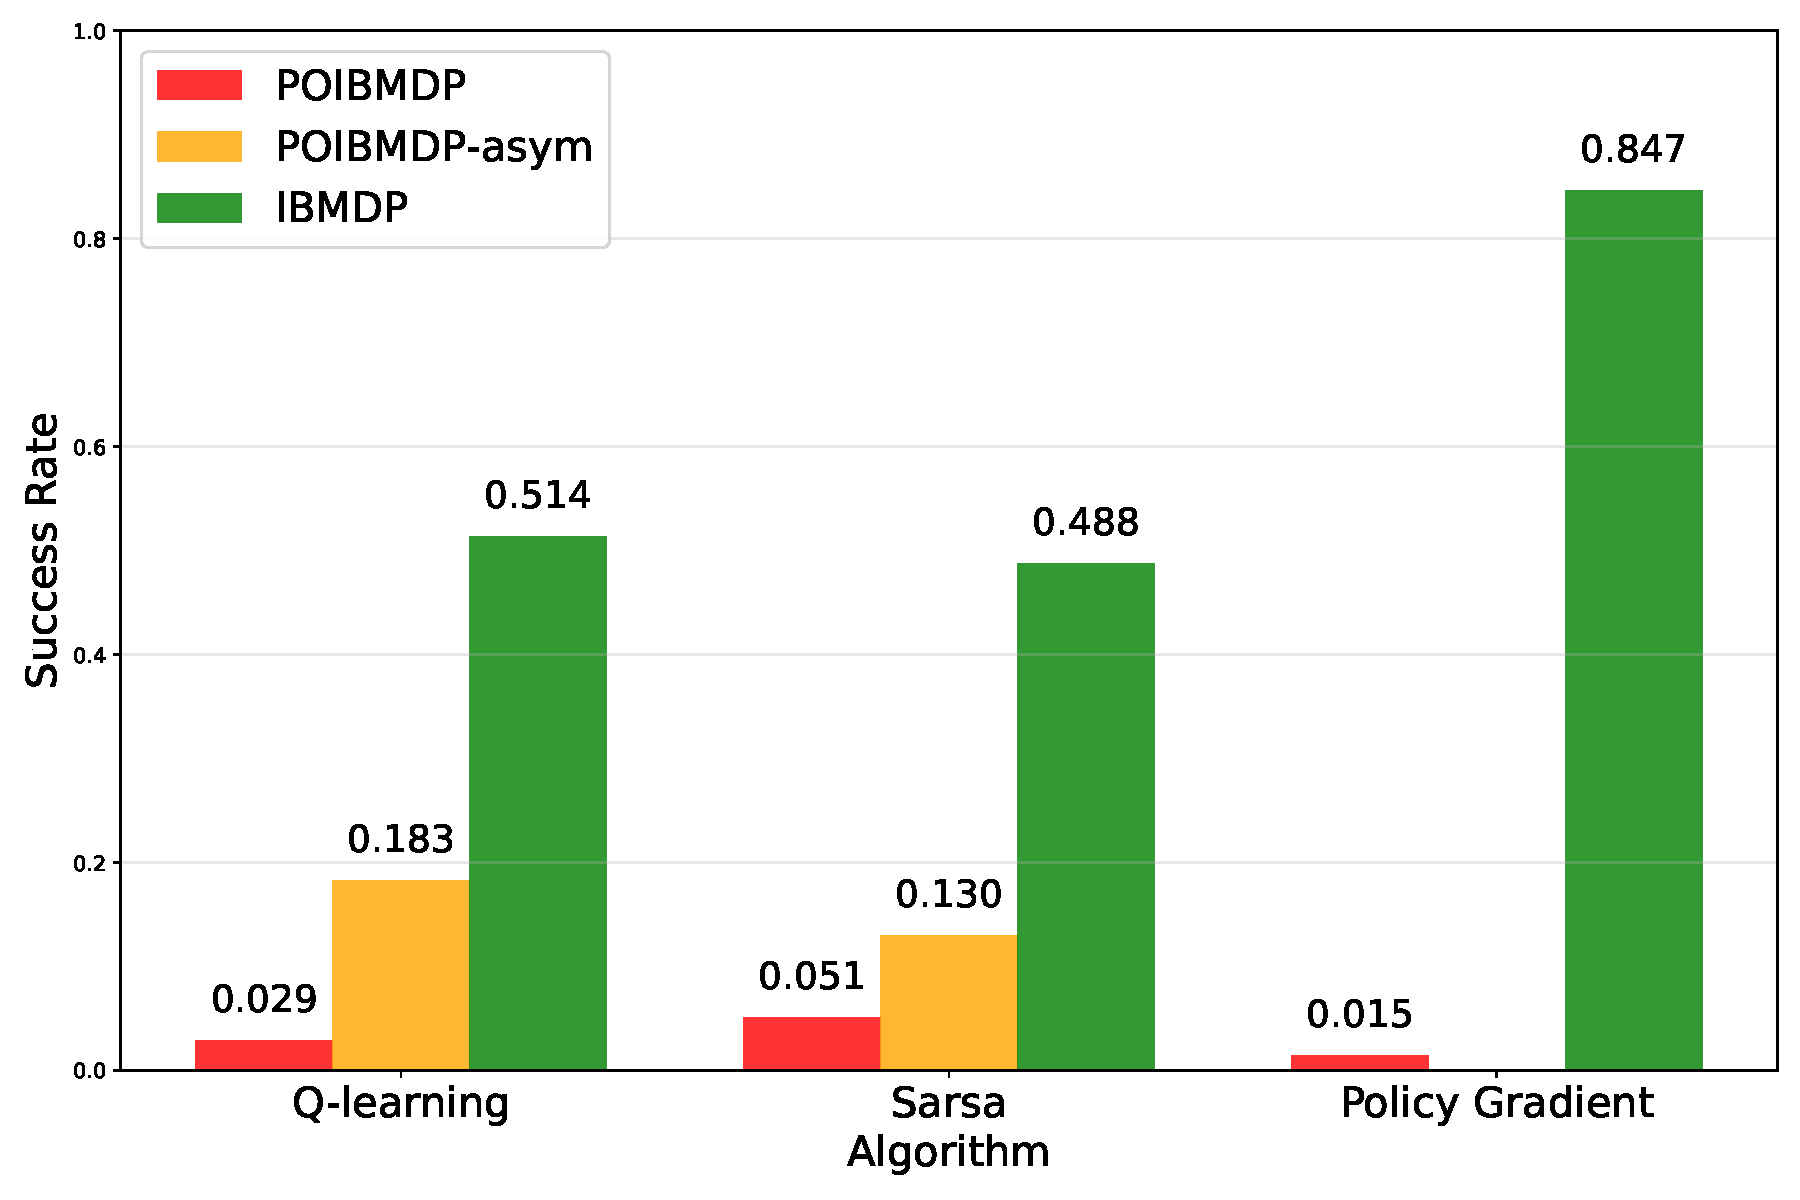
\includegraphics[width=0.8\textwidth]{images/images_part1/algorithm_performance_comparison_flattened.pdf}
    \caption{Success rates of different (asymmetric) RL algorithms over thousands of runs when applied to learning partially observable deterministic policies in a POIBMDP or learning deterministic policies in associated MDP and IBMDP.}\label{fig:po-vs-ib}
\end{figure}


\begin{figure}
    \begin{subfigure}[b]{0.49\textwidth}
        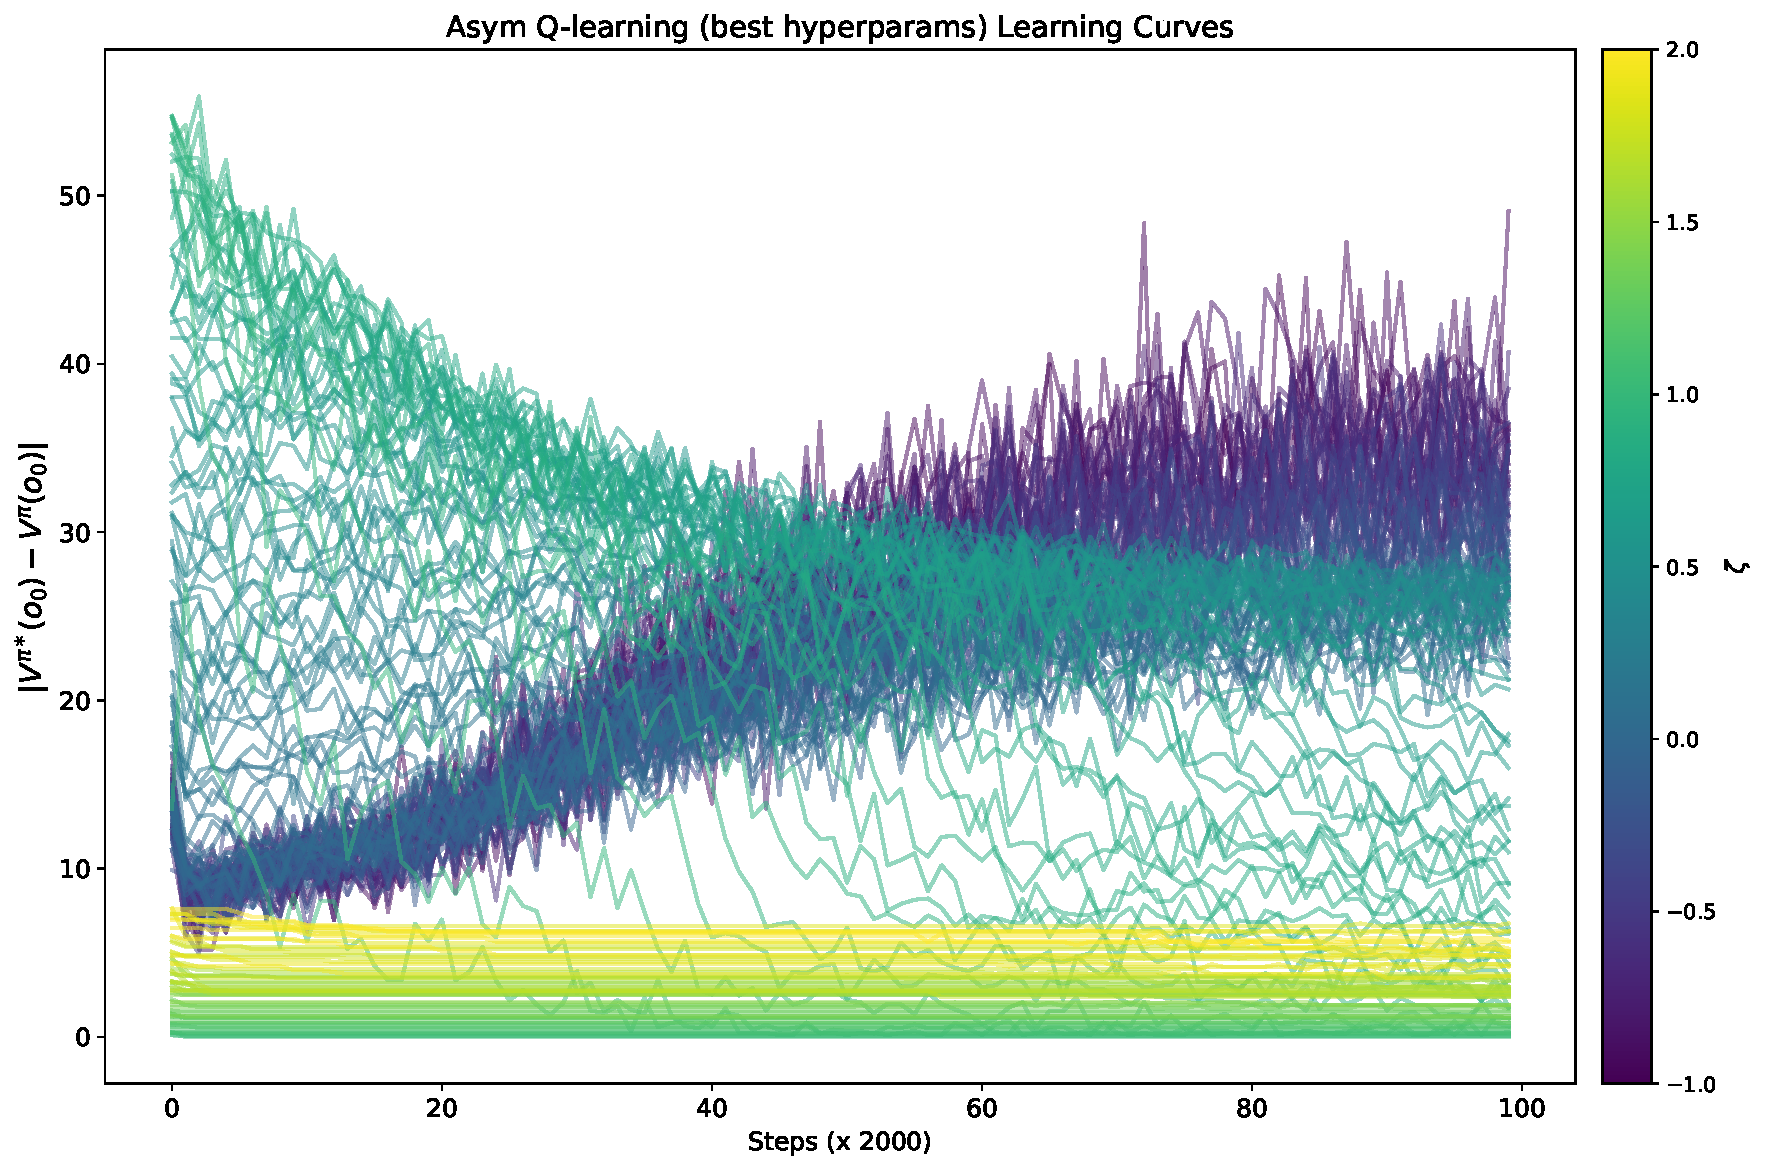
\includegraphics[width=\textwidth]{images/images_part1/ql_asym_best_learning_curves.pdf}
        \caption{Learning curves for asymmetric Q-learning with good hyperparameters.}
        \label{fig:best-learning-curves}
    \end{subfigure}
    \hfill
    \begin{subfigure}[b]{0.49\textwidth}
        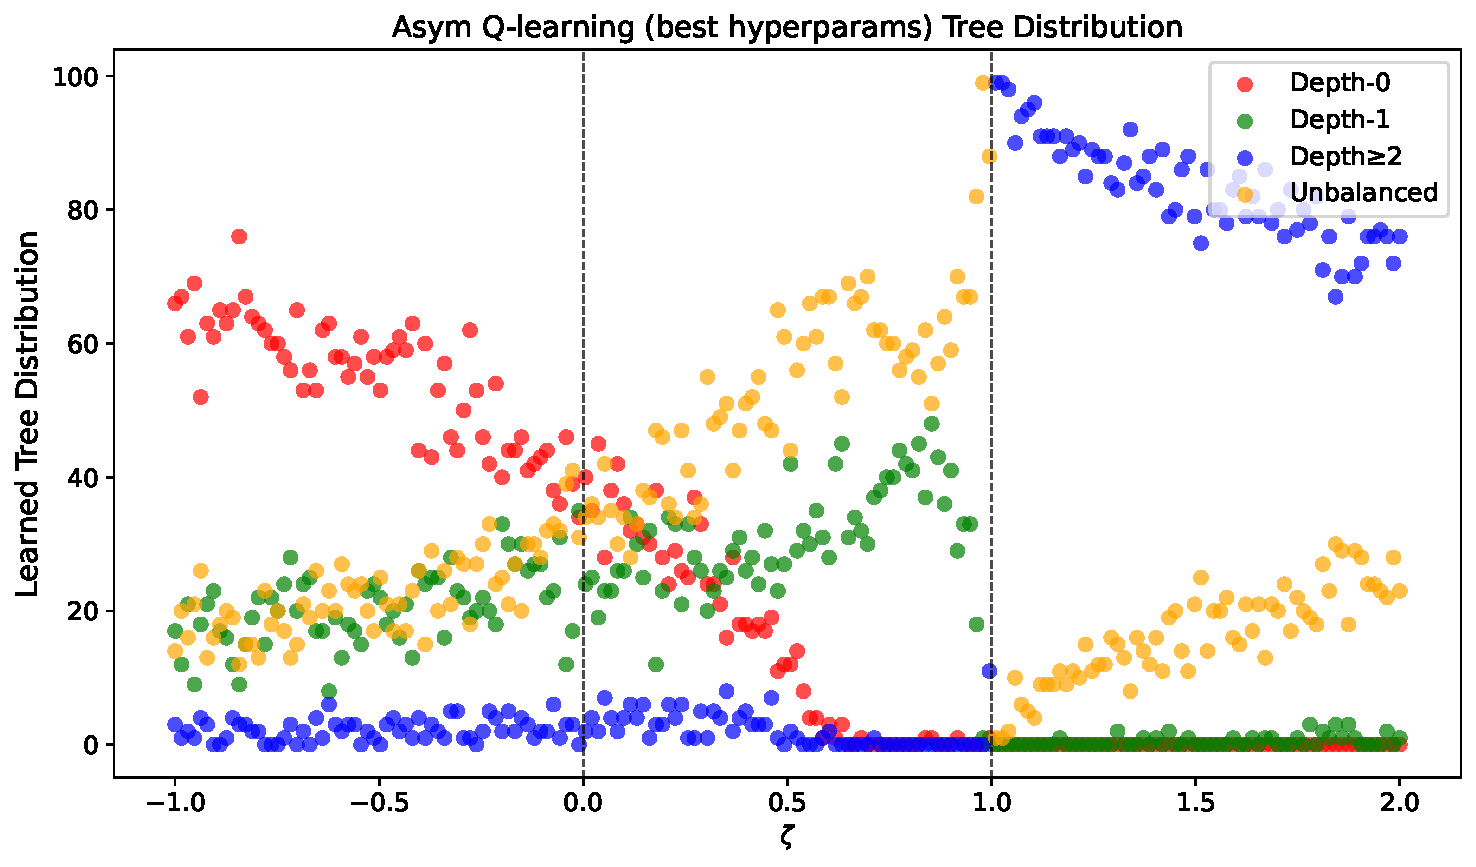
\includegraphics[width=\textwidth]{images/images_part1/ql_asym_best_tree_distributions.pdf}
        \caption{Trees distributions for asymmetric Q-learning with good hyperparameters}
        \label{fig:best-tree-distributions}
    \end{subfigure}
    \caption{Analysis of the top-performing asymmetric Q-learning instantiation. (left) Learning curves, and (right) tree distributions across different POIBMDP configurations.}
    \label{fig:asym-ql-analysis}
\end{figure}


\section{Conclusion}
In this Chapter, we have shown that direct learning of decision tree policies for MDPs can be reduced to learning deterministic partially observable policies in POMDPs that we called POIBMDPs.
By crafting a POIBMDP for which we know exactly the optimal deterministic partially observable policy, we were able to benchmark the sub-optimality of solutions learned with (asymmetric) reinforcement learning.

Across our experiments, we found that no algorithm could consistently learn a depth-1 decision tree policy for a grid world MDP despite it being optimal both in the POIBMDP and in the base MDP.

In the next chapter, we find that RL can find optimal deterministic partially observable policies for a special class of POIBMDPs that we believe makes for a convincing argument as to why learning in POIBMDP, i.e. direct learning of decision tree policies that optimize the RL objective (\ref{def:mdp-obj}) is so difficult.
